% !TEX spellcheck = en_US



% ~~~~~~~~~~~~~~~~~~~~~~~~~~~~~~~~~~~~~~~ V
% (NC) 2026 Haluk Bingol
% github.com/halukbingol/LaTeX-Templates
%
% Licensees may copy, distribute, display, and perform the work and make derivative works 
% and remixes based on it only for non-commercial purposes. 
% ~~~~~~~~~~~~~~~~~~~~~~~~~~~~~~~~~~~~~~~ A




% =====================================================================
%  Stacks -- Senior Level: The JVM, Concurrency and API Design
%  ---------------------------------------------------------------------
%  Built on hblib/Template/hblibTemplate.tex with the libraries in ../../hblib/.
%  Programs and their real outputs are in codeoutput/:
%     codeoutput/<Name>.java  a program (classes without main() are only compiled)
%     codeoutput/<Name>.sh    a terminal session, run in a copy of codeoutput/<Name>/
%     codeoutput/<Name>.txt   what it printed, made by:  bash run_examples.sh
% =====================================================================

\documentclass[aspectratio=169,10pt,compress]{beamer}

% ~~~~~~~~~~~~~~~~~~~~~~~~~~~~~~~~~~~~~~~~~~~~~~~~~~~~~~~~~~~~~~~~~ V hblib
	\usepackage{../../hblib/hblibPresentation} % lib presentation: theme, i/N, \hSection, algorithm2e, ...
	\usepackage{../../hblib/hblibCodeoutput} % lib code + output: \lstcode, \lstterminal, ...
	\usepackage{../../hblib/hblibDatastructures} % lib data structures: \hString, \hStack, \hQueue
% ~~~~~~~~~~~~~~~~~~~~~~~~~~~~~~~~~~~~~~~~~~~~~~~~~~~~~~~~~~~~~~~~~ A hblib


% xcolor, array (and the L{width} column), listings, tikz and algorithm2e come from the hblib libraries
\usepackage[T1]{fontenc}
\usepackage{lmodern}
\usepackage{booktabs}

\newcommand{\win}{\textbf{Windows}}
\newcommand{\mac}{\textbf{macOS}}

% algorithm2e set-up (the package is loaded by hblibPresentation)
\SetAlCapFnt{\small}
\SetAlCapNameFnt{\small}
\SetKwProg{Fn}{function}{}{end}
\SetKw{KwError}{error}

% ---------------------------------------------------------------------
\title{Stacks}
\subtitle{Senior Level: The JVM, Concurrency and API Design}
\author[Bingol]{Haluk O. Bingol}

\institute[FCIS]{
    Faculty of Computer and Information Sciences\\
    Yeditepe University
}
\date{
	{\tiny \hbTimeStamp}
}

\begin{document}




% ~~~~~~~~~~~~~~~~~~~~~~~~~~~~~~~~~~~~~~ V frm
\begin{frame}[t,fragile]
  \titlepage
\end{frame}
% ~~~~~~~~~~~~~~~~~~~~~~~~~~~~~~~~~~~~~~ A frm




% ~~~~~~~~~~~~~~~~~~~~~~~~~~~~~~~~~~~~~~ V frm
\begin{frame}[t,fragile] \frametitle{Outline}
  \begin{columns}[T]
    \begin{column}{0.48\textwidth}
      \tableofcontents[sections={1-3}, hideallsubsections]
    \end{column}
    \begin{column}{0.48\textwidth}
      \tableofcontents[sections={4-6}, hideallsubsections]
    \end{column}
  \end{columns}
\end{frame}
% ~~~~~~~~~~~~~~~~~~~~~~~~~~~~~~~~~~~~~~ A frm

% ~~~~~~~~~~~~~~~~~~~~~~~~~~~~~~~~~~~~~~ V
\hSection[JVM]{The JVM is a Stack Machine}
% ~~~~~~~~~~~~~~~~~~~~~~~~~~~~~~~~~~~~~~ A




% ~~~~~~~~~~~~~~~~~~~~~~~~~~~~~~~~~~~~~~ V frm
\begin{frame}[t,fragile] \frametitle{Bytecode works on an operand stack}
  \begin{columns}[T]
    \begin{column}{0.44\textwidth}
      \lstcode[basicstyle=\ttfamily\scriptsize]{codeoutput/Javap/Calc.java}{Java}
      \begin{itemize}\small
        \item \texttt{(a + b) * 2} in postfix is \texttt{a b + 2 *}
        \item that is exactly the bytecode
        \item \texttt{stack=2} (second method, \texttt{f}): \texttt{javac} computed the maximum depth
      \end{itemize}
    \end{column}
    \begin{column}{0.54\textwidth}
      \uncover<2->{\lstterminal[basicstyle=\ttfamily\tiny]{codeoutput/Javap.txt}}
    \end{column}
  \end{columns}
\end{frame}
% ~~~~~~~~~~~~~~~~~~~~~~~~~~~~~~~~~~~~~~ A frm




% ~~~~~~~~~~~~~~~~~~~~~~~~~~~~~~~~~~~~~~ V frm
\begin{frame}[t,fragile] \frametitle{Executing \texttt{f(3, 4)} step by step}
  \begin{center}\small
  \begin{tabular}{lll}
    \toprule
    \textbf{instruction} & \textbf{meaning}                         & \textbf{operand stack (top right)} \\
    \midrule
    \texttt{iload\_0}    & push local variable 0 (\texttt{a})       & 3 \\
    \texttt{iload\_1}    & push local variable 1 (\texttt{b})       & 3 4 \\
    \texttt{iadd}        & pop two ints, push the sum               & 7 \\
    \texttt{iconst\_2}   & push the constant 2                      & 7 2 \\
    \texttt{imul}        & pop two ints, push the product           & 14 \\
    \texttt{ireturn}     & pop and return to the caller             & (empty) \\
    \bottomrule
  \end{tabular}
  \end{center}
  \begin{itemize}\small
    \item A \textbf{stack machine} needs no register names: instructions are 1 byte, class files are small and portable.
    \item The JIT compiler (HotSpot C1/C2) turns this into register code for x64 or ARM (Apple silicon).
    \item The \emph{verifier} checks before running that no path can underflow or overflow the operand stack.
  \end{itemize}
\end{frame}
% ~~~~~~~~~~~~~~~~~~~~~~~~~~~~~~~~~~~~~~ A frm

% ~~~~~~~~~~~~~~~~~~~~~~~~~~~~~~~~~~~~~~ V
\hSection[Thread stacks]{Thread Stacks}
% ~~~~~~~~~~~~~~~~~~~~~~~~~~~~~~~~~~~~~~ A




% ~~~~~~~~~~~~~~~~~~~~~~~~~~~~~~~~~~~~~~ V frm
\begin{frame}[t,fragile] \frametitle{Two kinds of stack in every thread}
  \begin{columns}[T]
    \begin{column}{0.44\textwidth}
      \begin{center}
      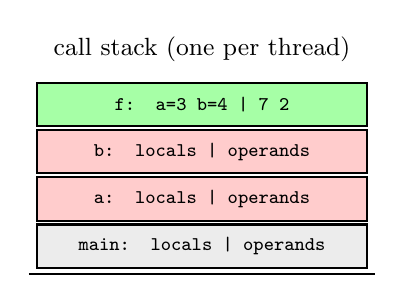
\begin{tikzpicture}[fr/.style={draw, thick, minimum width=4.2cm, minimum height=0.55cm, font=\ttfamily\scriptsize}]
        \node[fr, fill=gray!15]  at (0,0)   {main: locals | operands};
        \node[fr, fill=red!20]   at (0,0.6) {a: locals | operands};
        \node[fr, fill=red!20]   at (0,1.2) {b: locals | operands};
        \node[fr, fill=green!35] at (0,1.8) {f: a=3 b=4 | 7 2};
        \node[font=\small] at (0,2.5) {call stack (one per thread)};
        \draw[thick] (-2.2,-0.35) -- (2.2,-0.35);
      \end{tikzpicture}
      \end{center}
    \end{column}
    \begin{column}{0.52\textwidth}
      \begin{itemize}\small
        \item The \textbf{call stack} holds one \textbf{frame} per active method call.
        \item Each frame has its local variables and its own small \textbf{operand stack}.
        \item Its size is fixed when the thread starts: \texttt{-Xss} or \texttt{new Thread(group, task, name, stackSize)}.
        \item Objects live on the heap; the stack holds primitives and references.
        \item \emph{Escape analysis} lets the JIT keep some short-lived objects off the heap.
      \end{itemize}
    \end{column}
  \end{columns}
\end{frame}
% ~~~~~~~~~~~~~~~~~~~~~~~~~~~~~~~~~~~~~~ A frm




% ~~~~~~~~~~~~~~~~~~~~~~~~~~~~~~~~~~~~~~ V frm
\begin{frame}[t,fragile] \frametitle{How deep can we go? \texttt{-Xss}}
  \begin{columns}[T]
    \begin{column}{0.36\textwidth}
      \lstcode[basicstyle=\ttfamily\tiny]{codeoutput/Xss/Depth.java}{Java}
    \end{column}
    \begin{column}{0.62\textwidth}
      \uncover<2->{\lstterminal[basicstyle=\ttfamily\tiny]{codeoutput/Xss.txt}}
    \end{column}
  \end{columns}
  \small The depth grows with the stack size; the exact numbers depend on the frame size and the JIT. \texttt{ThreadStackSize} is in KB.
  \texttt{-Xss} works the same on \win{} and \mac.
\end{frame}
% ~~~~~~~~~~~~~~~~~~~~~~~~~~~~~~~~~~~~~~ A frm




% ~~~~~~~~~~~~~~~~~~~~~~~~~~~~~~~~~~~~~~ V frm
\begin{frame}[t,fragile] \frametitle{Looking at the call stack from Java}
  \lstcoderightstep[0.62][basicstyle=\ttfamily\tiny][basicstyle=\ttfamily\tiny]{codeoutput/Walker.java}{Java}{codeoutput/Walker.txt}

  \vspace{0.2em}
  \small \texttt{StackWalker} (Java 9) walks the frames lazily, top first. Logging frameworks and security checks use it to find their caller.
\end{frame}
% ~~~~~~~~~~~~~~~~~~~~~~~~~~~~~~~~~~~~~~ A frm




% ~~~~~~~~~~~~~~~~~~~~~~~~~~~~~~~~~~~~~~ V frm
\begin{frame}[t,fragile] \frametitle{Virtual threads: stacks on the heap}
  \lstcoderightstep[0.62][basicstyle=\ttfamily\tiny][basicstyle=\ttfamily\tiny]{codeoutput/Virtual.java}{Java}{codeoutput/Virtual.txt}

  \vspace{0.2em}
  \small Java 21 virtual threads keep their frames in \textbf{heap} objects that grow and shrink: 100\,000 of them are cheap.
\end{frame}
% ~~~~~~~~~~~~~~~~~~~~~~~~~~~~~~~~~~~~~~ A frm

% ~~~~~~~~~~~~~~~~~~~~~~~~~~~~~~~~~~~~~~ V
\hSection[Concurrency]{Stacks and Threads}
% ~~~~~~~~~~~~~~~~~~~~~~~~~~~~~~~~~~~~~~ A




% ~~~~~~~~~~~~~~~~~~~~~~~~~~~~~~~~~~~~~~ V frm
\begin{frame}[t,fragile] \frametitle{A data race}
  \begin{columns}[T]
    \begin{column}{0.49\textwidth}
      \lstcode[basicstyle=\ttfamily\tiny, lastline=17]{codeoutput/Race.java}{Java}
    \end{column}
    \begin{column}{0.49\textwidth}
      \lstcode[basicstyle=\ttfamily\tiny, firstline=18, firstnumber=18]{codeoutput/Race.java}{Java}
    \end{column}
  \end{columns}
\end{frame}
% ~~~~~~~~~~~~~~~~~~~~~~~~~~~~~~~~~~~~~~ A frm




% ~~~~~~~~~~~~~~~~~~~~~~~~~~~~~~~~~~~~~~ V frm
\begin{frame}[t,fragile] \frametitle{A data race: the result}
  \begin{columns}[T]
    \begin{column}{0.56\textwidth}
      \lstoutput[basicstyle=\ttfamily\tiny]{codeoutput/Race.txt}
    \end{column}
    \begin{column}{0.40\textwidth}
      \begin{itemize}\small
        \item \texttt{a[size++] = x} is read, add, write: two threads can read the same \texttt{size} and overwrite each other.
        \item The number lost changes from run to run. It is a bug even in a run where it happens to be 0.
        \item \texttt{Stack} locks every call; \texttt{ConcurrentLinkedDeque} uses compare-and-set: both are correct.
      \end{itemize}
    \end{column}
  \end{columns}
\end{frame}
% ~~~~~~~~~~~~~~~~~~~~~~~~~~~~~~~~~~~~~~ A frm




% ~~~~~~~~~~~~~~~~~~~~~~~~~~~~~~~~~~~~~~ V frm
\begin{frame}[t,fragile] \frametitle{Choices for a stack shared by threads}
  \begin{center}\footnotesize
  \begin{tabular}{lL{0.28\textwidth}L{0.32\textwidth}}
    \toprule
    \textbf{Option}                          & \textbf{How}                            & \textbf{Cost} \\
    \midrule
    \texttt{java.util.Stack}                 & every method \texttt{synchronized}      & a lock on every call; compound actions still unsafe \\
    \texttt{synchronized} wrapper / own lock & one lock around \emph{your} operations   & you choose what is atomic \\
    \texttt{ConcurrentLinkedDeque}           & lock-free linked nodes (CAS)            & no blocking; \texttt{size()} is $O(n)$ \\
    \texttt{LinkedBlockingDeque}             & lock; \texttt{takeFirst} waits when empty & producer/consumer hand-off \\
    one stack per thread                     & no sharing at all                       & usually the fastest \\
    \bottomrule
  \end{tabular}
  \end{center}
  \small \hRemark{Compound actions}: \texttt{if (!s.isEmpty()) s.pop()} can fail even on a synchronized \texttt{Stack}: another thread may pop in between.
\end{frame}
% ~~~~~~~~~~~~~~~~~~~~~~~~~~~~~~~~~~~~~~ A frm




% ~~~~~~~~~~~~~~~~~~~~~~~~~~~~~~~~~~~~~~ V frm
\begin{frame}[t,fragile] \frametitle{A lock-free stack: Treiber 1986}
  \begin{columns}[T]
    \begin{column}{0.56\textwidth}
      \lstcode[basicstyle=\ttfamily\tiny]{codeoutput/TreiberStack.java}{Java}
    \end{column}
    \begin{column}{0.4\textwidth}
      \begin{itemize}\small
        \item \texttt{compareAndSet(old, fresh)}: set \texttt{top} to \texttt{fresh} \textbf{only if} it is still \texttt{old}, in one atomic CPU instruction.
        \item If another thread changed \texttt{top}, retry with the new value.
        \item No thread ever waits for a lock: \emph{lock-free}.
        \item Nodes are immutable (a \texttt{record}).
      \end{itemize}
    \end{column}
  \end{columns}
\end{frame}
% ~~~~~~~~~~~~~~~~~~~~~~~~~~~~~~~~~~~~~~ A frm




% ~~~~~~~~~~~~~~~~~~~~~~~~~~~~~~~~~~~~~~ V frm
\begin{frame}[t,fragile] \frametitle{Testing it under contention}
  \begin{columns}[T]
    \begin{column}{0.49\textwidth}
      \lstcode[basicstyle=\ttfamily\tiny, lastline=15]{codeoutput/TreiberTest.java}{Java}
    \end{column}
    \begin{column}{0.49\textwidth}
      \lstcode[basicstyle=\ttfamily\tiny, firstline=16, firstnumber=16]{codeoutput/TreiberTest.java}{Java}
    \end{column}
  \end{columns}
\end{frame}
% ~~~~~~~~~~~~~~~~~~~~~~~~~~~~~~~~~~~~~~ A frm




% ~~~~~~~~~~~~~~~~~~~~~~~~~~~~~~~~~~~~~~ V frm
\begin{frame}[t,fragile] \frametitle{Testing it: the result}
  \begin{columns}[T]
    \begin{column}{0.5\textwidth}
      \lstoutput[basicstyle=\ttfamily\scriptsize]{codeoutput/TreiberTest.txt}
    \end{column}
    \begin{column}{0.46\textwidth}
      \begin{itemize}\small
        \item 8 threads push $1 \dots 100\,000$ each; 4 of them also pop after every push.
        \item The sum of everything popped plus what is left equals the sum pushed: nothing lost, nothing duplicated.
        \item A passing test does not prove a concurrent program correct; it can only find bugs. Tools: \texttt{jcstress} (OpenJDK).
      \end{itemize}
    \end{column}
  \end{columns}
\end{frame}
% ~~~~~~~~~~~~~~~~~~~~~~~~~~~~~~~~~~~~~~ A frm




% ~~~~~~~~~~~~~~~~~~~~~~~~~~~~~~~~~~~~~~ V frm
\begin{frame}[t,fragile] \frametitle{The ABA problem}
  \begin{enumerate}\small
    \item Thread 1 reads \texttt{top = A} (with \texttt{A.next = B}) and is paused.
    \item Thread 2 pops \texttt{A}, pops \texttt{B}, pushes \texttt{A} again: \texttt{top = A}, but \texttt{A.next} is now different.
    \item Thread 1 resumes: \texttt{compareAndSet(A, B)} succeeds, because \texttt{top} is ``still'' \texttt{A}. \texttt{B} is back on the stack: corrupted.
  \end{enumerate}
  \begin{block}{In Java}
    \small Our \texttt{TreiberStack} creates a \textbf{new} node for every push, and the garbage collector never reuses a node that a thread
    still references, so step 2 cannot bring back the same \texttt{A}. In C or C++ with node reuse (free lists) ABA is real: fixes are
    tagged pointers (\texttt{AtomicStampedReference} in Java), hazard pointers or epochs.
  \end{block}
\end{frame}
% ~~~~~~~~~~~~~~~~~~~~~~~~~~~~~~~~~~~~~~ A frm

% ~~~~~~~~~~~~~~~~~~~~~~~~~~~~~~~~~~~~~~ V
\hSection[Security]{Robustness and Security}
% ~~~~~~~~~~~~~~~~~~~~~~~~~~~~~~~~~~~~~~ A




% ~~~~~~~~~~~~~~~~~~~~~~~~~~~~~~~~~~~~~~ V frm
\begin{frame}[t,fragile] \frametitle{Untrusted input and deep nesting}
  \begin{columns}[T]
    \begin{column}{0.49\textwidth}
      \lstcode[basicstyle=\ttfamily\tiny, lastline=22]{codeoutput/Nesting.java}{Java}
    \end{column}
    \begin{column}{0.49\textwidth}
      \lstcode[basicstyle=\ttfamily\tiny, firstline=23, firstnumber=23]{codeoutput/Nesting.java}{Java}
    \end{column}
  \end{columns}
\end{frame}
% ~~~~~~~~~~~~~~~~~~~~~~~~~~~~~~~~~~~~~~ A frm




% ~~~~~~~~~~~~~~~~~~~~~~~~~~~~~~~~~~~~~~ V frm
\begin{frame}[t,fragile] \frametitle{Deep nesting: the result}
  \begin{columns}[T]
    \begin{column}{0.56\textwidth}
      \lstoutput[basicstyle=\ttfamily\tiny]{codeoutput/Nesting.txt}
    \end{column}
    \begin{column}{0.40\textwidth}
      \begin{itemize}\small
        \item A recursive parser lets the \emph{input} decide how deep the call stack goes: a \textbf{denial-of-service} attack with 200 KB of brackets.
        \item An explicit stack on the heap survives, and a \textbf{limit} rejects the input early with a clear message.
        \item Real parsers do this: Jackson limits JSON nesting to 1000 levels by default (since version 2.15).
      \end{itemize}
    \end{column}
  \end{columns}
\end{frame}
% ~~~~~~~~~~~~~~~~~~~~~~~~~~~~~~~~~~~~~~ A frm




% ~~~~~~~~~~~~~~~~~~~~~~~~~~~~~~~~~~~~~~ V frm
\begin{frame}[t,fragile] \frametitle{Checklist for stacks in production code}
  \begin{itemize}
    \item \textbf{Bound} every stack that input can grow: a maximum depth or size, with a clear error.
    \item Prefer \textbf{iteration with an explicit stack} to recursion when the depth depends on data.
    \item Catch \texttt{StackOverflowError} only at a boundary (one request), never to ``continue as usual'': the state may be inconsistent.
    \item Do not \textbf{loiter}: null out popped slots, or use \texttt{ArrayDeque}, which does.
    \item Do not share a non-thread-safe stack; if you must, choose a concurrent structure on purpose.
    \item Stack traces in error pages leak class names and versions: log them, do not show them to users.
  \end{itemize}
\end{frame}
% ~~~~~~~~~~~~~~~~~~~~~~~~~~~~~~~~~~~~~~ A frm

% ~~~~~~~~~~~~~~~~~~~~~~~~~~~~~~~~~~~~~~ V
\hSection[API design]{API Design Lessons}
% ~~~~~~~~~~~~~~~~~~~~~~~~~~~~~~~~~~~~~~ A




% ~~~~~~~~~~~~~~~~~~~~~~~~~~~~~~~~~~~~~~ V frm
\begin{frame}[t,fragile] \frametitle{25 years of stacks in the JDK}
  \lstcoderightstep[0.6][basicstyle=\ttfamily\tiny][basicstyle=\ttfamily\tiny]{codeoutput/Sequenced.java}{Java}{codeoutput/Sequenced.txt}

  \vspace{0.2em}
  \small Java 21's \texttt{SequencedCollection} adds \texttt{reversed()}, \texttt{getFirst()}, \texttt{getLast()} to both. Note that \texttt{Stack}
  still lets anyone insert and remove in the \textbf{middle}.
\end{frame}
% ~~~~~~~~~~~~~~~~~~~~~~~~~~~~~~~~~~~~~~ A frm




% ~~~~~~~~~~~~~~~~~~~~~~~~~~~~~~~~~~~~~~ V frm
\begin{frame}[t,fragile] \frametitle{What went wrong with \texttt{java.util.Stack}}
  \begin{columns}[T]
    \begin{column}{0.48\textwidth}
      \begin{block}{Java 1.0 (1996)}
        \small \texttt{class Stack<E> extends Vector<E>}
        \begin{itemize}\small
          \item \textbf{inheritance} instead of composition: all 40+ \texttt{Vector} methods are public
          \item iteration is bottom first, \texttt{search} counts from the top
          \item every call is synchronized, even in one thread
        \end{itemize}
      \end{block}
    \end{column}
    \begin{column}{0.48\textwidth}
      \begin{block}{Java 6 (2006): \texttt{Deque}}
        \small \texttt{interface Deque<E>}, \texttt{class ArrayDeque<E>}
        \begin{itemize}\small
          \item an \textbf{interface}: many implementations
          \item but a deque also allows \texttt{addLast}, \texttt{pollLast}: still not a pure stack
          \item two sets of methods (throw / return special value)
        \end{itemize}
      \end{block}
    \end{column}
  \end{columns}
  \vspace{0.3em}
  \small Lesson (J. Bloch, \emph{Effective Java}, ``favor composition over inheritance''): a class that \emph{has} a list
  can enforce LIFO; a class that \emph{is} a list cannot. A pure stack type is still a good wrapper to write yourself.
\end{frame}
% ~~~~~~~~~~~~~~~~~~~~~~~~~~~~~~~~~~~~~~ A frm

% ~~~~~~~~~~~~~~~~~~~~~~~~~~~~~~~~~~~~~~ V
\hSection[Summary]{Summary}
% ~~~~~~~~~~~~~~~~~~~~~~~~~~~~~~~~~~~~~~ A




% ~~~~~~~~~~~~~~~~~~~~~~~~~~~~~~~~~~~~~~ V frm
\begin{frame}[t,fragile] \frametitle{Big ideas}
  \begin{itemize}
    \item The JVM itself is a stack machine; bytecode is postfix, checked by the verifier.
    \item Every thread has a call stack of frames; its size is fixed (\texttt{-Xss}) except for virtual threads.
    \item Shared stacks need synchronization; \texttt{compareAndSet} gives lock-free stacks (Treiber), with ABA in mind.
    \item Input-controlled depth is an attack surface: explicit stacks with limits.
    \item Design: composition over inheritance; document empty, \texttt{null}, order and thread safety.
  \end{itemize}
\end{frame}
% ~~~~~~~~~~~~~~~~~~~~~~~~~~~~~~~~~~~~~~ A frm




% ~~~~~~~~~~~~~~~~~~~~~~~~~~~~~~~~~~~~~~ V frm
\begin{frame}[t,fragile] \frametitle{Projects}
  \begin{enumerate}\small
    \item Write \texttt{BoundedStack<T>} that \emph{has} an \texttt{ArrayDeque}, exposes only stack operations, has a maximum size, and is thread safe. Test it with 8 threads.
    \item Benchmark \texttt{TreiberStack}, \texttt{ConcurrentLinkedDeque} and a \texttt{synchronized} \texttt{ArrayDeque} with 1, 2, 4, 8 threads using JMH.
    \item Write a postfix interpreter that compiles \texttt{(a + b) * c} into your own ``bytecode'' and runs it on an operand stack with a computed maximum depth.
    \item Make the \texttt{Nesting} recursive parser safe without removing the recursion (a depth counter). Compare with the stack version.
    \item Reproduce ABA in Java with \texttt{AtomicReference} and a pool of reused nodes; fix it with \texttt{AtomicStampedReference}.
  \end{enumerate}
\end{frame}
% ~~~~~~~~~~~~~~~~~~~~~~~~~~~~~~~~~~~~~~ A frm




% ~~~~~~~~~~~~~~~~~~~~~~~~~~~~~~~~~~~~~~ V frm
\begin{frame}[t,fragile]
	\begin{center}
		\vspace{4cm}
		\hRemark{\Huge Questions?}
	\end{center}
\end{frame}
% ~~~~~~~~~~~~~~~~~~~~~~~~~~~~~~~~~~~~~~ A frm



\end{document}
